%!TEX root = ../../../adrien_gomar_phd.tex

The outlet isentropic Mach number is $0.99$ for an inlet Mach number of $0.4$. 
This case, for which experimental uncertainties are available, 
has been largely addressed in the literature by
\citet{Sbardella2001,Duta2002,Campobasso2003} and \citet{Cinnella2004}. 
This test case is challenging in terms of non-linearities as a separation bubble and a shock are present.

Steady results of the isentropic Mach number are shown in
Fig.~\ref{fig:stcf11_rans_transonic}.  For this flow regime,
a small separation
bubble develops on the suction side at the leading edge~(cf.~Fig.~\ref{fig:stcf11_transonic_field_mis_bw}).  The flow then accelerates, followed by a passage shock.  
The experimental data suggests that the shock appears
sooner on the suction side than in the computations; all the results 
reported in the literature exhibit similar discrepancies (see
Refs.~\cite{Fransson1999,Sbardella2001,Duta2002,Campobasso2003,Cinnella2004}). 
Otherwise, the present results are in fair agreement with experimental data.
\begin{figure}[htb]
  \centering
  \begin{minipage}[b]{.46\linewidth}
    \centering
    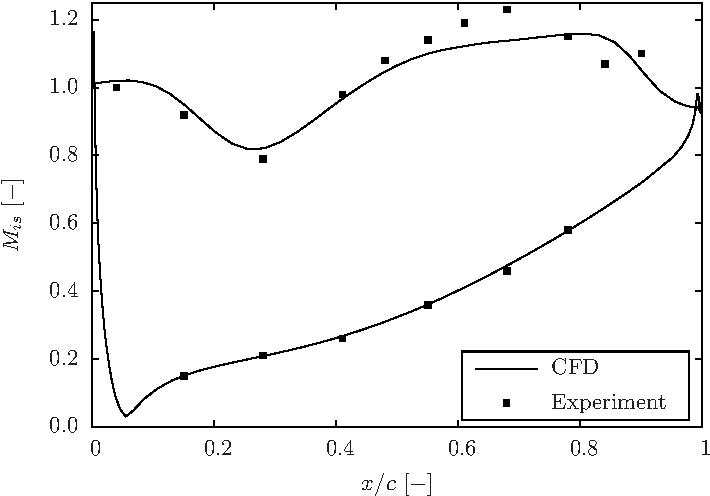
\includegraphics[width=\textwidth]{STCF11_RANS_TRANSONIC.pdf}
    \caption{Steady results of the isentropic Mach number at blade
      wall, transonic case}
    \label{fig:stcf11_rans_transonic}
  \end{minipage}\quad
  \begin{minipage}[b]{.46\linewidth}
    \centering
    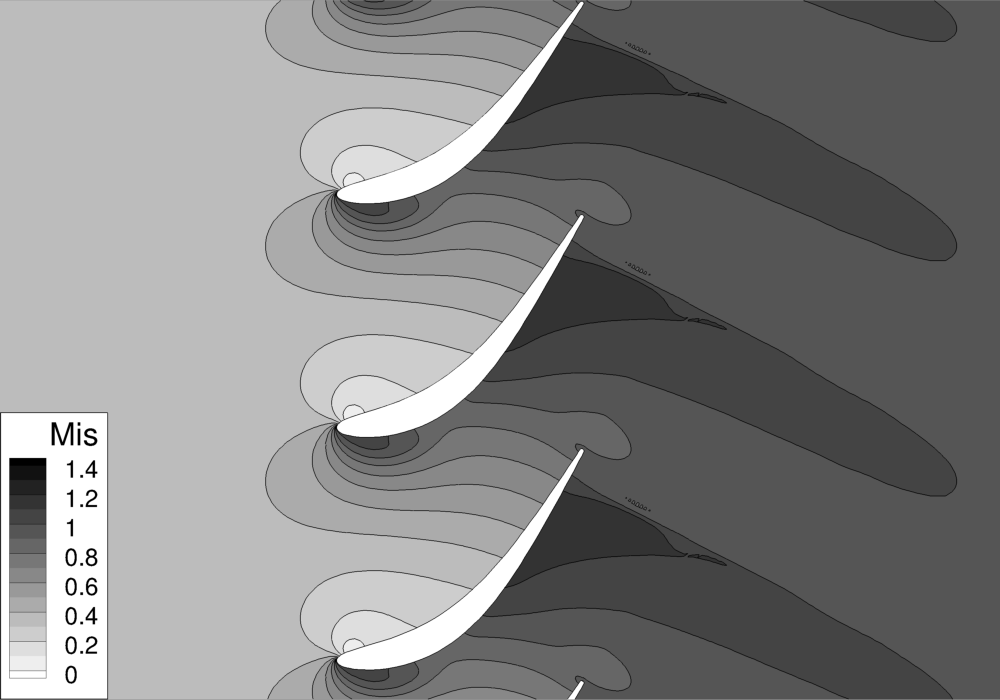
\includegraphics[width=\textwidth]{STCF11_TRANSONIC_FIELD_MIS_BW.png}
    \caption{Steady isentropic Mach number contours, transonic case}
    \label{fig:stcf11_transonic_field_mis_bw}
  \end{minipage}
\end{figure}

% unsteady results
The aeroelastic experimental data are compared to the present results
obtained with both the DTS and the HB approach.  Considering the opposite phase vibration case (the 10\textsuperscript{th} nodal diameter), 
the amplitude and the
phase of the pressure coefficient are presented in
Fig.~\ref{fig:stcf11_ael_transonic_ibpa_180_paper}. Also plotted are the results of
Cinnella~\emph{et~al.}~\cite{Cinnella2004}, computed with a non-linear viscous
approach using the Spalart-Allmaras turbulence model. The present HB and the DTS
results are superimposed, which indicates that the one harmonic HB solution is able
to reproduce the unsteady non-linear effects without increasing the
number of harmonics. This observation is only valid near the wall,
before the harmonics are created naturally by the flow, due to the
non-linear effects. The results are in good agreement with
the experimental data and display the same trends as that of
\citet{Cinnella2004}. A slight discrepancy can be observed within the shock
region, where the amplitude and the phase phenomena are predicted
further than the experiments indicate.  This can be attributed to the poor
prediction of the shock position and hence the poor prediction
of its interaction with the motion of the blade.
\begin{figure}[htb]
  \centering
  \begin{tabular}{cc}
    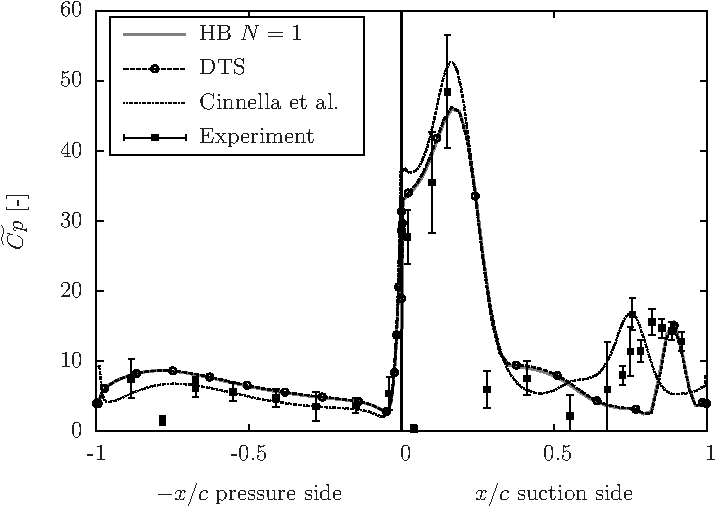
\includegraphics[width=.45\textwidth]{STCF11_AEL_TRANSONIC_IBPA_180_Cp_paper.pdf}
    &
    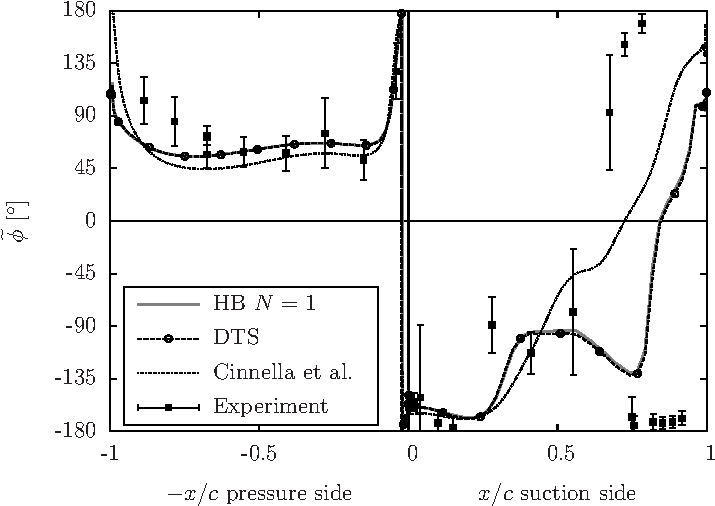
\includegraphics[width=.45\textwidth]{STCF11_AEL_TRANSONIC_IBPA_180_Phi_paper.pdf}\\
    (a) Amplitude part & Phase part
  \end{tabular}
  \caption{Wall pressure harmonic analysis for an opposite phase vibration, transonic case}
  \label{fig:stcf11_ael_transonic_ibpa_180_paper}
\end{figure}

The results for the $-2$\textsuperscript{th} nodal diameter are also shown in
Fig.~\ref{fig:stcf11_ael_transonic_ibpa_324_paper}. Again,
the HB results are superimposed on the DTS ones. Moreover, these are in
good agreement with the experiments, considering the uncertainties of
the experimental data.
\begin{figure}[htb]
  \centering 
  \begin{tabular}{cc}
    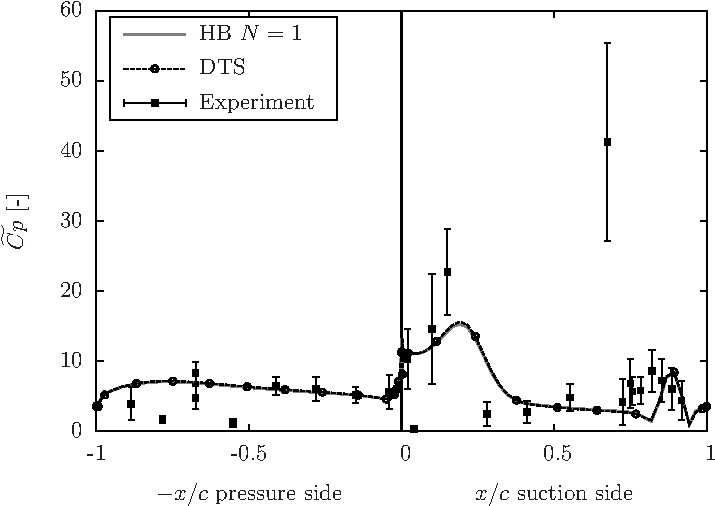
\includegraphics[width=.45\textwidth]{STCF11_AEL_TRANSONIC_IBPA_324_Cp_paper.pdf}
    &
    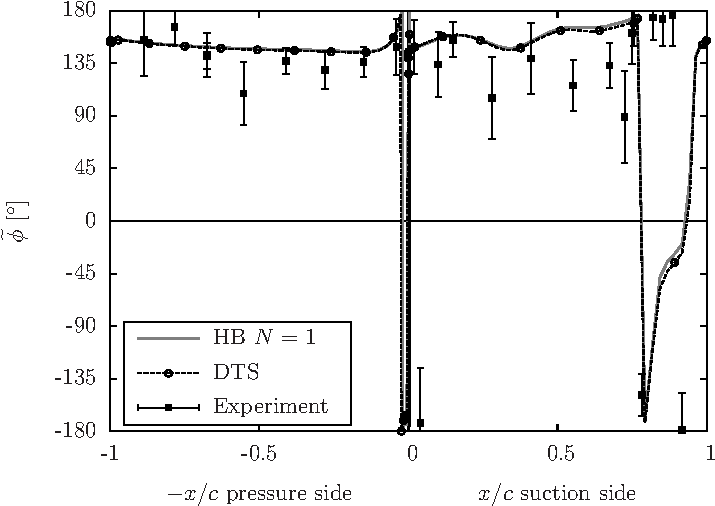
\includegraphics[width=.45\textwidth]{STCF11_AEL_TRANSONIC_IBPA_324_Phi_paper.pdf}\\
    (a) Amplitude part & (b) Phase part
  \end{tabular}
  \caption{Wall pressure harmonic analysis for \mbox{$n_d=-2$}, transonic case}
  \label{fig:stcf11_ael_transonic_ibpa_324_paper}
\end{figure}

The damping is shown in Fig.~\ref{fig:stcf11_transonic_damping} for
the transonic case. Also plotted are the results from
\citet{Fransson1999} (potential code), and 
from \citet{Cinnella2004} (RANS). The scattering is much more severe
than for the subsonic case. The trends obtained with the RANS approaches are similar. However, the
discrepancies between the two RANS codes are significant in terms of
levels.
Recently, \citet{Vogt:2011fk} reported similar discrepancies 
for damping predictions of subsonic and transonic cascades, 
showing that the damping can be significantly affected by 
small local changes in the amplitude and/or the phase.
\begin{figure}[htb]
  \centering
  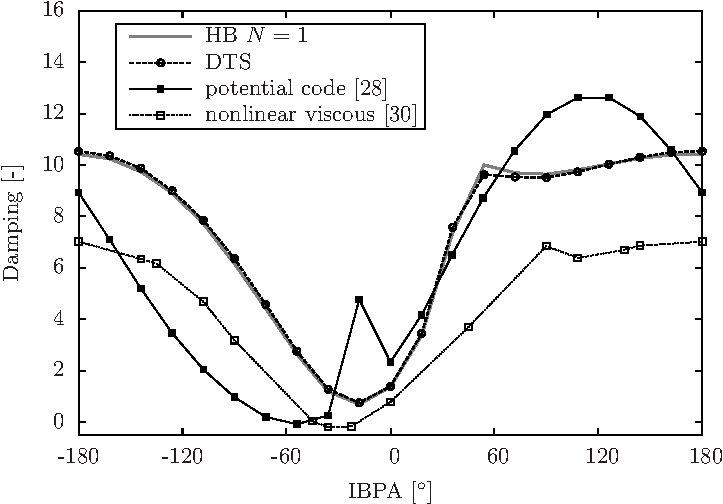
\includegraphics[width=.46\linewidth]{STCF11_TRANSONIC_DAMPING.pdf}
  \caption{Aerodynamic damping coefficient versus IBPA, transonic
    case}
  \label{fig:stcf11_transonic_damping}
\end{figure}
In terms of computational efficiency, the HB method is 7 times faster
than the DTS  for all the IBPAs.